\documentclass[12pt]{beamer}

% INCLUDE GRAPHICS
\usepackage{graphicx}

% TABLES
\newcommand{\ra}[1]{\renewcommand{\arraystretch}{#1}} % spaces in tables
\usepackage{booktabs}   % Allows the use of \toprule, \midrule and \bottomrule in tables for horizontal lines

% FONTS
% PdfLatex
% \usepackage[T1]{fontenc}
% \usepackage{pgf}
% \logo{\pgfputat{\pgfxy(-1,-0.435)}{\pgfbox[center,base]{
\includegraphics[width=1.2cm,natwidth=610,natheight=642]{KUNATLogo.pdf}}}}

% FONTS
% xelatex
\usepackage{fontspec}
% \fontspec[Path=../fonts/,]{
%     UprightFont = *-regular,
%     ItalicFont = *-italic,
%     Boldfont = *-bold
% }

% NOTE
% Add fonts to ~/.fonts for this to work
% \setsansfont{TeX Gyre Heros}
% \setsansfont{TeX Gyre Heros Cn}
% \setsansfont{Liberation Sans}
\setsansfont{Muli}
% \setsansfont{Helvetica Neue}

% Monospaces font
\setmonofont{Monaco}

% Use serif for Math environments
\usefonttheme[onlymath]{serif}

% TODO Use mono fonts

% CODE
\usepackage{listings} % Code block (source code) \begin{lstlisting}
\lstset{
    language=Python,                        % Code langugage
    commentstyle=\color{gray},              % Comments font
    basicstyle=\scriptsize\ttfamily,             % Code font, Examples: \footnotesize, \ttfamily
    keywordstyle=\bfseries\color{blue},
    stringstyle=\color{orange},
    numbers=left,                           % Line nums position
    numberstyle=\tiny,                      % Line-numbers fonts
    stepnumber=1,                           % Step between two line-numbers
    numbersep=5pt,                          % How far are line-numbers from code
    numbers=none,
    frame=lines,                             % A frame around the code
    rulecolor=\color{gray},
    tabsize=4,                              % Default tab size
    captionpos=b,                           % Caption-position = bottom
    breaklines=true,                        % Automatic line breaking?
    breakatwhitespace=false,                % Automatic breaks only at whitespace?
    showspaces=false,                       % Dont make spaces visible
    showstringspaces=false,                 % Dont make spaces visible in strings
    showtabs=false,                         % Dont make tabls visible
    belowskip=5pt,
    morekeywords={range, xrange},
    backgroundcolor=\color{white}
    % emph={[2]root,base}
    % morekeywords={one,two,three,four,five,six,seven,eight,
}

\newcommand{\code}[1]{{\small\ttfamily #1}} % \code{inline code}

%
% COLORS
%
\definecolor{kugreen}{RGB}{50,93,61}

\definecolor{orange}{RGB}{255,127,0}
\definecolor{green}{RGB}{0,153,51}
\definecolor{blue}{RGB}{3,115,187}
\definecolor{red}{RGB}{221,17,68}
\definecolor{gray}{RGB}{55,55,55}
\definecolor{black}{RGB}{0,0,0}

\definecolor{offwhite}{RGB}{249,242,215}
\definecolor{foreground}{RGB}{23,23,23}
\definecolor{background}{RGB}{255,255,255}
\definecolor{subtitle}{RGB}{102,255,204}
\definecolor{hilight}{RGB}{102,255,204}
\definecolor{vhilight}{RGB}{255,111,207}
\definecolor{lolight}{RGB}{155,155,155}


%
% BEAMER STYLE COLORS
%
\setbeamercolor{titlelike}{fg=black}
\setbeamercolor{subtitle}{fg=blue}
\setbeamercolor{institute}{fg=gray}
\setbeamercolor{normal text}{fg=foreground,bg=background}
\setbeamercolor{item}{fg=foreground} % color of bullets
\setbeamercolor{subitem}{fg=gray}
\setbeamercolor{itemize/enumerate subbody}{fg=gray}

\setbeamerfont{itemize/enumerate subbody}{size=\footnotesize}
\setbeamerfont{itemize/enumerate subitem}{size=\footnotesize}

\setbeamerfont{footnote}{size=\tiny}

\setbeamersize{text margin left=10pt}
\setbeamersize{text margin right=10pt}
\setbeamersize{sidebar width right=0pt}
\setbeamersize{sidebar width left=0pt}

%
% REMOVES THE NAVIGATION BAR
%
\beamertemplatenavigationsymbolsempty


% BEAMER TEMPLATES


%
% BEAMER BACKGROUND
%
\usebackgroundtemplate{

    \rule{0pt}{0.97\paperheight}%
    \hspace*{1.15\paperwidth}%
    \makebox[0pt][r]{%
        
\includegraphics[width=100pt,natwidth=610,natheight=642]{KUNATLogo.pdf}
    }

}


%
% BEAMER HEADLINE
%
\setbeamertemplate{headline}{}


%
% BEAMER TITLE
%
\setbeamertemplate{frametitle}
{
    \begin{centering}
    \insertframetitle\par
    \end{centering}
}


%
% BEAMER FOOTER
%
\setbeamertemplate{footline}[text line]
{%
    \vbox{%
        \insertvrule{0.5pt}{kugreen}

        \vspace{2pt}

        \strut{
        % \rmfamily\itshape
        \expandafter\insertshorttitle
        \expandafter\insertauthor
        \insertshortinstitute
        }
        \hfill\strut{
        }
        \hfill\strut{
            \insertframenumber\,/\,\inserttotalframenumber
        }

        \vspace{1pt}
    }
}


%
% TITLE PAGE
%
% \setbeamertemplate{title page}
% {
%     % Remove beamer background
%     \setbeamertemplate{background}{}
% 
%     \begin{beamercolorbox}[center]{beamer color}
% 
%         {
%             \huge
%             \color{kugreen}
%             \inserttitle
%         }
%         \bigskip
%         \bigskip
% 
%         % 
\includegraphics[width=2cm]{KUNATLogo}
% 
%         \bigskip
%         {
%             \bf
%             \rmfamily
%             {\large \insertauthor}
%         }
% 
%         \smallskip
%         {
%             \rmfamily
%             \footnotesize
%             \insertinstitute
%         }
% 
%         {
%             \rmfamily
%             \footnotesize
%             \insertdate
%         }
% 
%     \end{beamercolorbox}
% 
%     % Do not count the title page
%     \addtocounter{framenumber}{-1}
% }


\usepackage{soul}

\title[]{Week 5\\Molecular Statistics}


\institute[, University of Copenhagen]{C315B\\ Department of Chemistry \\ University of Copenhagen}

\author[J. C. Kromann]{Jimmy Charnley Kromann}

\date{
    \code{\scriptsize help: jimmy@charnley.dk}
}




% ===============
% begin slides
% ===============


\begin{document}

{
\usebackgroundtemplate{}
\begin{frame}[plain]
    \titlepage
    \addtocounter{framenumber}{-1}
\end{frame}
}

\begin{frame}[fragile]

    \frametitle{Week 5, Overview}

    Useful python for bachelor/future science

\end{frame}


\begin{frame}[fragile]

    \frametitle{Plot the data}

    \begin{align*}
        \Delta G^\circ = \Delta U - T \Delta S^\circ + \Delta W + \delta
    \end{align*}

    \begin{columns}[t]

        \column{0.5\linewidth}

            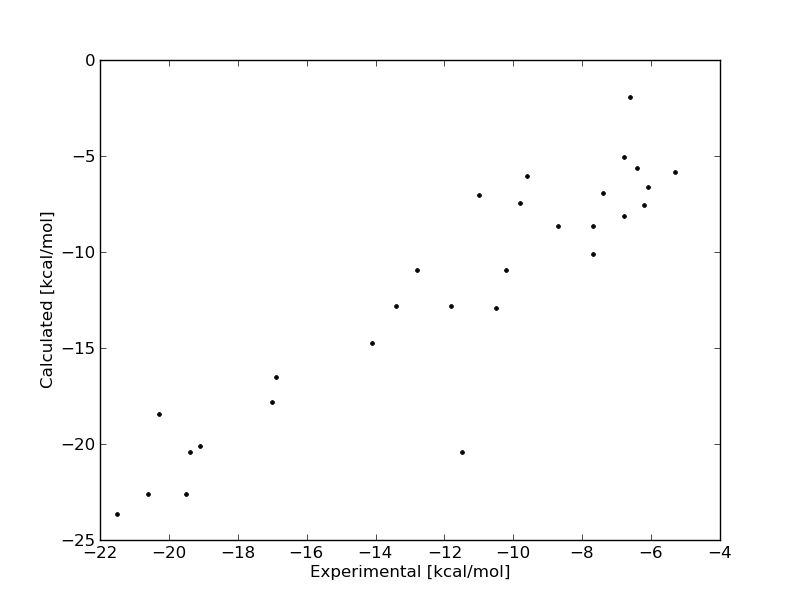
\includegraphics[width=1.1\textwidth]{images/binding_energy.png}

        \column{0.4\linewidth}

            Columns:\newline ID, $\Delta U$, $\Delta W$, $\Delta S^\circ$\newline

            $\delta = -5.83$, $T = 298.0$

    \end{columns}

\end{frame}


\begin{frame}[fragile]

    \frametitle{Analyse the data}

    \begin{itemize}
        \item Calculate the Root-mean-square deviation (RMSD)

        \begin{align*}
            \mathrm{RMSD} = \sqrt{\frac{\sum_i^N (x_{\mathrm{exp},i}-x_{\mathrm{cal},i})^2 }{N}}
        \end{align*}

    \end{itemize}

    \begin{itemize}
        \item Calculate the Pearson Correlation factor $r$ and corresponding $p$ value.
    \end{itemize}

    \bigskip

    Hint: There {\bf might} be a Pearson function in the \code{scipy} module.

\end{frame}


\begin{frame}[fragile]

    \frametitle{Print the data}

    Format the output of the python script

\begin{lstlisting}
print "{0:5d}".format(42)
\end{lstlisting}

\smallskip

\begin{lstlisting}
"{0:5d}".format(42) # integer
"{0:5.2f}".format(65.6789) # float
"{0:5s}".format("hello") # string
\end{lstlisting}

\bigskip

Format the output for a latex table

\smallskip

\begin{lstlisting}
print "{0:5d} & {1:5.2f} & {2:5.2f} \\\\".format(i, G_exp[i], G_cal[i])
\end{lstlisting}

\bigskip

https://docs.python.org/3/library/string.html\#formatspec

\end{frame}


\begin{frame} 
    \frametitle{15min break}
    \begin{center}
        
\includegraphics[width=0.6\textwidth]{images/barbie3.png}
    \end{center}
\end{frame}


\begin{frame}[fragile]

    % http://www.eveandersson.com/pi/monte-carlo-circle
    % How this program works:
    %
    % If a circle of radius R is inscribed inside a square with side length 2R,
    % then the area of the circle will be pi*R^2 and the area of the square
    % will be (2R)^2.
    % So the ratio of the area of the circle to the area of the square will be
    % pi/4.
    %
    % This means that, if you pick N points at random inside the square,
    % approximately N*pi/4 of those points should fall inside the circle.
    %
    % This program picks points at random inside the square.
    % It then checks to see if the point is inside the circle (it knows it's
    % inside the circle if x^2 + y^2 < R^2, where x and y are the coordinates
    % of the point and R is the radius of the circle).
    % The program keeps track of how many points it's picked so far (N) and how
    % many of those points fell inside the circle (M).
    %
    % Pi is then approximated as follows:
    %
    %           4*M
    %      pi = ---
    %            N
    %
    % Although the Monte Carlo Method is often useful for solving
    % problems in physics and mathematics which cannot be solved by
    % analytical means, it is a rather slow method of calculating
    % pi.
    % To calculate each significant digit there will have to be
    % about 10 times as many trials as to calculate the preceding
    % significant digit.

    \frametitle{Monte Carlo $\pi$}

    \begin{columns}[c]

        \column{0.5\linewidth}

            \begin{align*}
                % A_\text{circle} &= \pi \cdot r^2 \\
                % A_\text{square} &= 4 \\
                % r &= 1 \\
                \pi &= 4 \cdot A_\text{circle} / A_\text{square}
            \end{align*}

            \begin{equation*}
                x^2 + y^2 < r^2
            \end{equation*}

        \column{0.5\linewidth}

            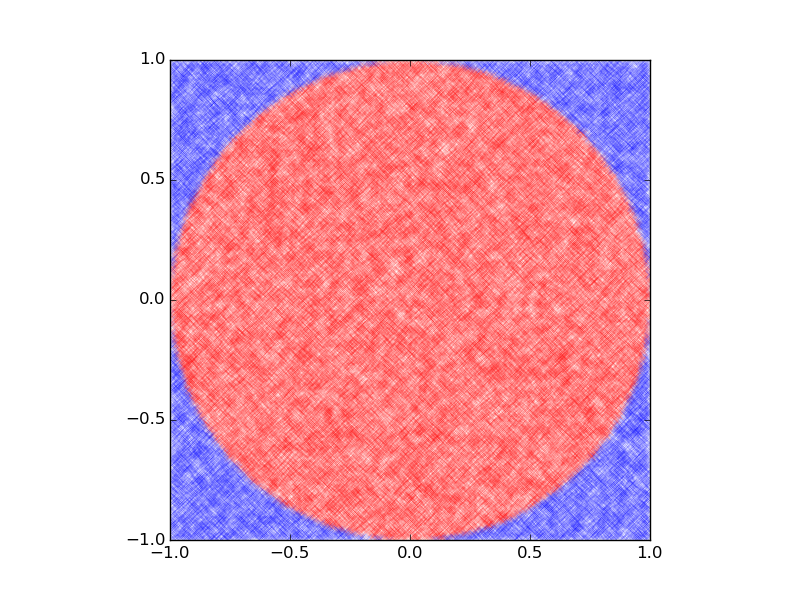
\includegraphics[width=1.1\textwidth]{images/circle.png}

    \end{columns}

        \begin{itemize}
            \item Calculate Pi.
            \item How many points before converge?
        \end{itemize}

    % \bigskip
    %
    % \small
    % https://en.wikipedia.org/wiki/Monte\_Carlo\_integration


\end{frame}

{
\usebackgroundtemplate{

    \rule{0pt}{1.0\paperheight}%
    \hspace*{1.15\paperwidth}%
    \makebox[-8pt][r]{%
        
\includegraphics[width=250pt]{images/cry.jpg}%
    }

}

\begin{frame}[fragile]
    \frametitle{Debug}

    \begin{columns}[c]

        \column{0.5\linewidth}
            Let us do some more debug

        \column{0.5\linewidth}

    \end{columns}

\end{frame}

}

%%%%%%%%%%%%%%%%%%%%%%%%%%%%%%%%%%%%%%%%%%%%%%%%%%%%%%%%%%%%%%%%%%%%%%
%% END FRAMES
%%%%%%%%%%%%%%%%%%%%%%%%%%%%%%%%%%%%%%%%%%%%%%%%%%%%%%%%%%%%%%%%%%%%%%

\end{document}

